\chapter{Architektura aplikacji}
W rozdziale przedstawiono wymagania funkcjonalne i niefunkcjonalne, które zostały postawione aplikacji. Zaprezentowano również diagramy przypadków użycia, stanów oraz sekwencji.
\section{wymagania funkcjonalne}
Wymagania funkcjonalne określają zachowanie systemu i jego reakcji na określone zadania \cite{Wymagania}. Stanowią one podstawę dla wykonawcy oprogramowania do opracowania odpowiednich metod oraz funkcjonalności. Precyzyjne zdefiniowanie wymagań z perspektywy biznesowej pozwala na dopasowanie tworzonych rozwiązań do potrzeb organizacji oraz celów strategicznych projektu. Takie rozwiązanie umożliwia wdrożenie systemu zgodnego z oczekiwaniami zleceniodawcy.

\begin{longtable}{|c|p{5cm}|p{8cm}|}
	\caption{Wymagania funkcjonalne systemu do zarządzania budżetem domowym}
	\label{tab:wymagania_funkcjonalne} \\
	\hline
	\textbf{Nr} & \textbf{Wymaganie funkcjonalne} & \textbf{Opis} \\ \hline
	
	1. & Rejestracja użytkownika & System umożliwia utworzenie konta użytkownika z danymi logowania. \\ \hline
	2. & Logowanie do systemu & System weryfikuje dane użytkownika i umożliwia dostęp do panelu aplikacji. \\ \hline
	3. & Sprawdzenie dostępnych środków & Użytkownik może sprawdzić ile posiada balansu na koncie. \\ \hline
	4. & Wpłata pieniędzy na konto & Użytkownik może zasilić konto. \\ \hline
	5. & Przegląd historii wydatków & Aplikacja wyświetla listę wszystkich wydatków. \\ \hline
	6. & Tworzenie przelewu & System pozwala stworzyć przelew użytkownikowi. \\ \hline
	7. & Podsumowanie finansów konta & Użytkownik może sprawdzić dane o swoich wydatkach dla danego konta. \\ \hline
	8. & Kategoryzowanie transakcji & Użytkownik może podać kategorię dla wpłat i wypłat z konta. \\ \hline
	9. & Prezentacja wydatków na wykresie & System wyświetla wykres z wydatkami za dzień, tydzień, miesiąc oraz rok. \\ \hline
\end{longtable}

\section{Wymagania niefunkcjonalne}
Wymaganiami niefunkcjonalnymi nazywamy wszystkie potrzeby, które nie odnoszą się bezpośrednio do funkcjonalności produktu, lecz określają jego właściwości jakościowe \cite{Wymagania}. Dotyczą one m.in. takich zagadnień jak czas reakcji systemu, termin dostarczenia produktu, wyglądu interfejsu użytkownika, czy bezpieczeństwa. Stanowią kluczowy element dla wykonawcy oprogramowania, przy projektowaniu architektury, doborze technologii oraz planowaniu procesu wdrożenia. Mają istotne znaczenie z perspektywy biznesowej, ponieważ wpływają na satysfakcję użytkowników, konkurencyjność systemu oraz koszty jego utrzymania. Dla zamawiających gwarantują odpowiednią jakość, stabilność i wydajność oprogramowania. 

\begin{longtable}{|c|p{3.1cm}|p{9.9cm}|}
		\caption{Wymagania niefunkcjonalne systemu do zarządzania budżetem domowym}
	\label{tab:wymagania_niefunkcjonalne} \\
	\hline
	\textbf{Nr} & \textbf{Wymaganie niefunkcjonalne} & \textbf{Opis} \\ \hline
	
	1. & Niezawodność & System w krótkim czasie odzyskuje pełną funkcjonalność w przypadku wystąpienia błędu. \\ \hline
	2. & Dostępność & System ma być dostępna przez 99.5\% czasu działania serwera.\\ \hline
	3. & Wydajność & System reaguje na żądanie w czasie krótszym niż 1 sekunda. Może obsłużyć do 1000 użytkowników jednocześnie. System jest w stanie przetworzyć do 10 GB na godzinę.  System jest skalowalny.\\ \hline
	4. & Bezpieczeństwo & System zapewnia, że dane są dostępne tylko dla osób upoważnionych. Autoryzacja użytkowników odbywa się poprzez podanie odpowiedniego loginu oraz hasła. Hasła muszą być przechowywane w formie zaszyfrowanej. \\ \hline
	5. & Wdrożenie & Aplikacja serwerowa musi być uruchomiona w środowisku JVM oraz korzystać z wersji Java 21 , Warstwa prezentacji uruchamiana w środowisku NodeJs z wykorzystaniem 9 wersji biblioteki React. Dane przechowywane w postaci dokumentów bazy danych MongoDB w wersji 8, Aplikacja uruchomiana jest w środowisku systemu operacyjnego Windows 11 oraz Linux \\ \hline
	
\end{longtable}


\section{Diagramy UML}
Jednym z kluczowych etapów w procesie tworzenia oprogramowanie jest wizualizacja systemu \cite{UML}. Język UML (ang. \textit{Unified Modeling Language}), czyli ujednolicony język modelowania nie jest językiem programowani, chociaż może uprościć proces tworzenia aplikacji generując kod na podstawie diagramów. UML definiuje dwie podstawowe składowe: notację elementów na diagramach oraz ich semantykę \cite{UML1}. W artykule T. Sobestańczyk diagram opisany jest słowami ,,Diagram jest schematem przedstawiającym zbiór bytów''.
\section{TODO:Diagramy przypadków użycia}
Diagram przypadków użycia (ang. \textit{Use Case Diagram}) prezentuje usługi, które system świadczy aktorom, bez wskazywania rozwiązań technologicznych \cite{UML1}. Stanowi on podstawę do modelowania szczegółowych części systemu.
\textbf{TODO: Diagram został utworzony na zajęciach laboratoryjnych i nie zostaną wykorzystane z niego wszystkie funkcjonalności. Dodatkowo jest duży i nieczytelny. Podmienie go w miarę możliwości na diagram bardziej czytelny i zwięzły. Pozostałe diagramy najprawdopodobniej mają taką samą pozycję.}
\begin{figure}[H]
	\centering
	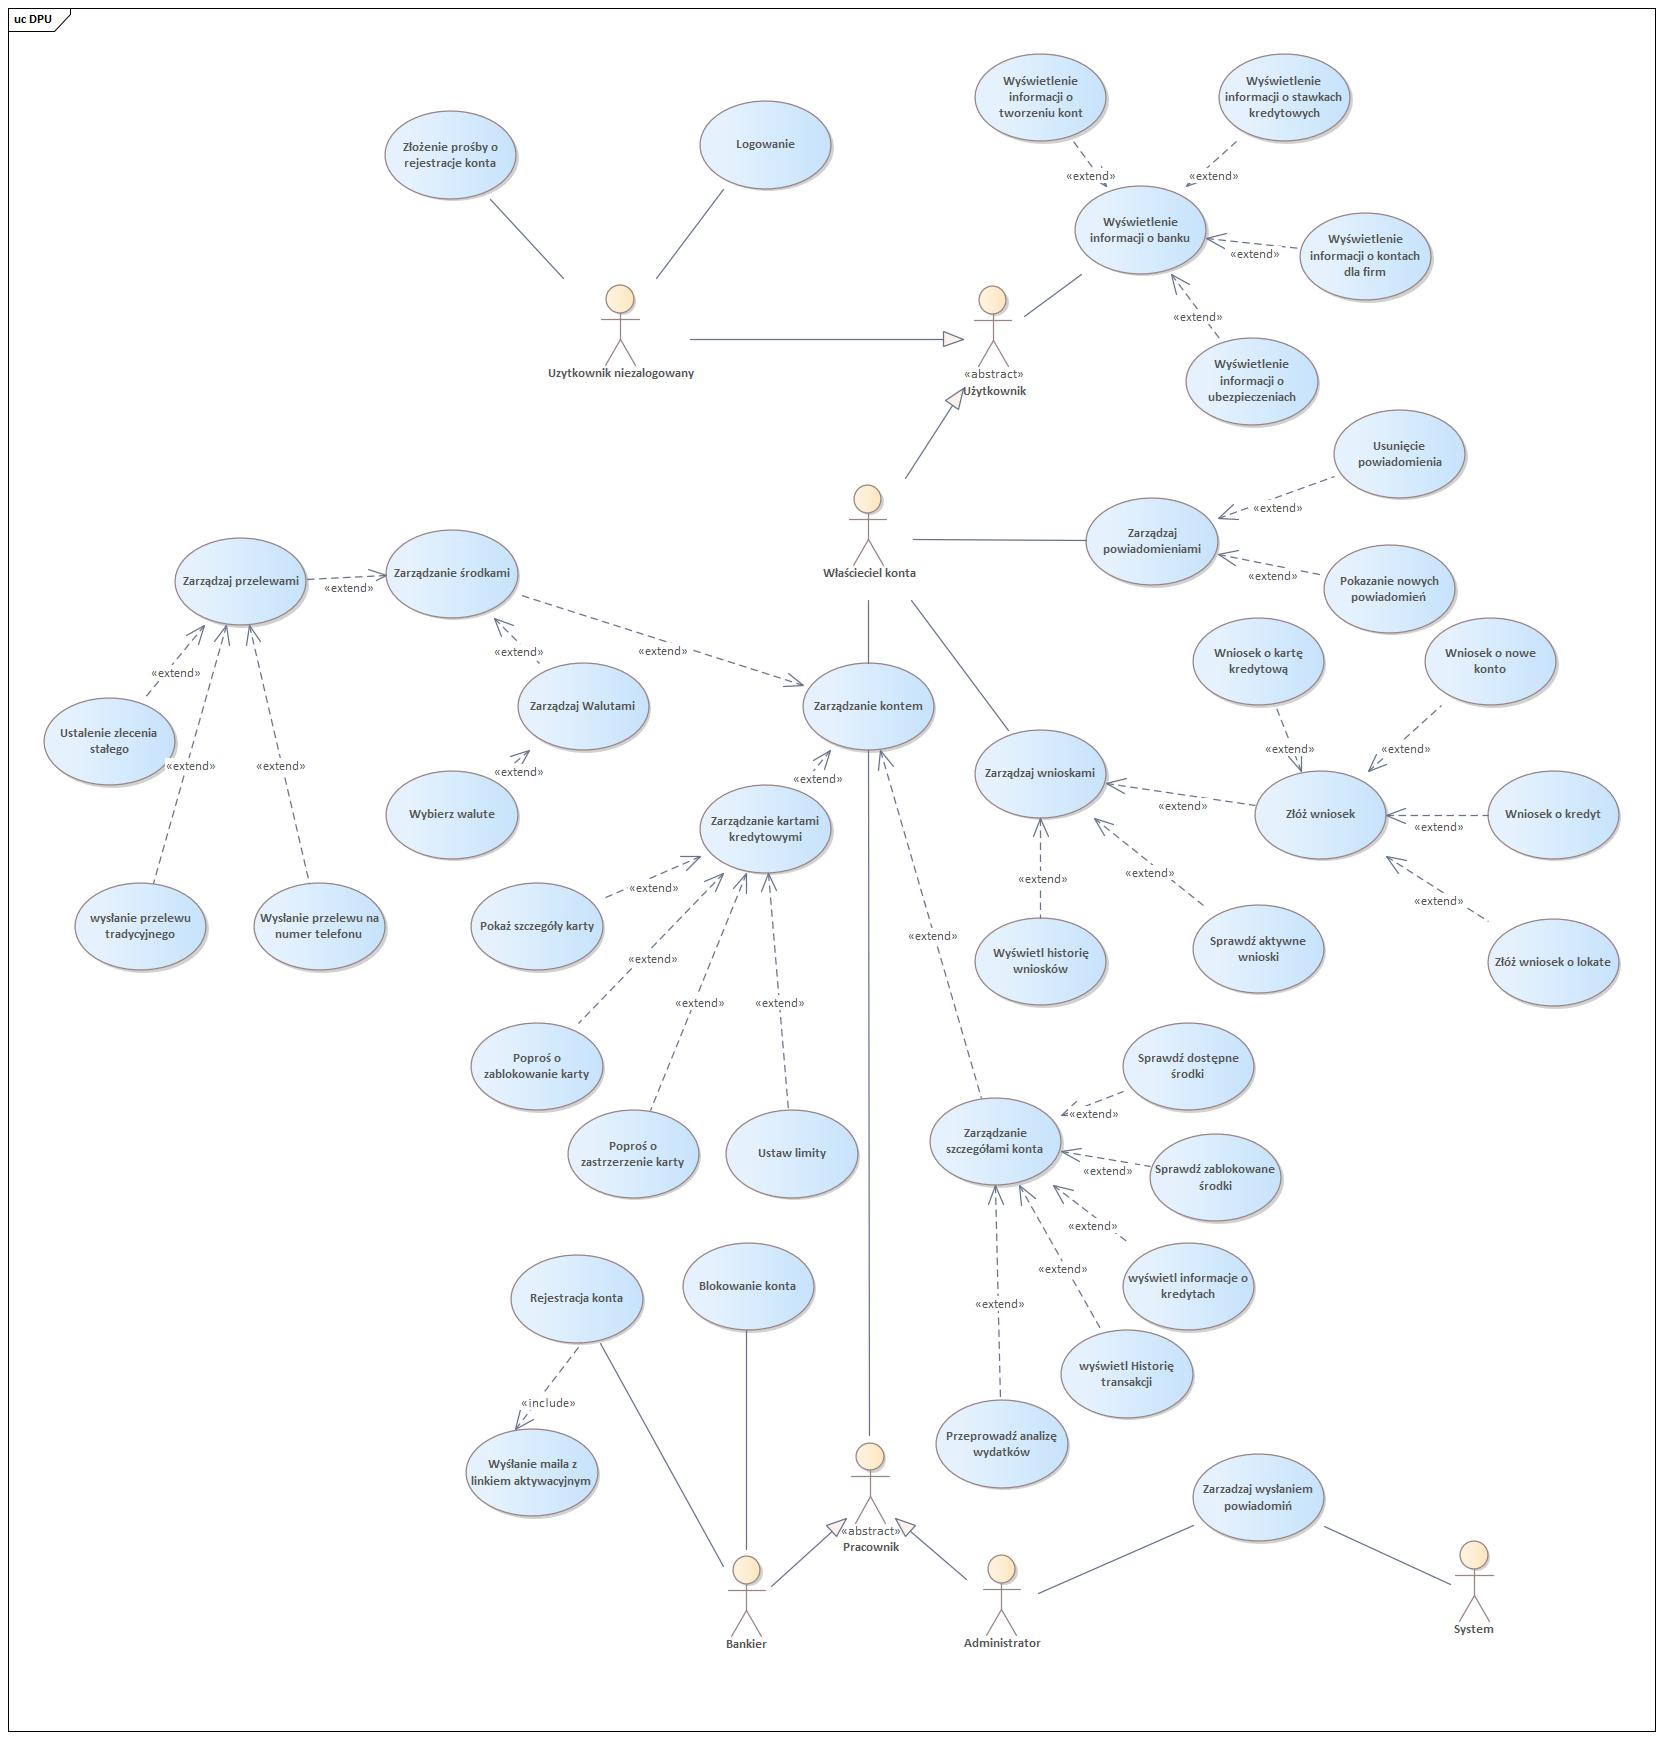
\includegraphics[width=1\textwidth]{images/DPU.jpg}
	\caption{Diagram przypadków użycia}
	\label{fig:UseCase}
\end{figure}
\section{Diagram stanów}
Diagram maszyny stanów (ang. \textit{state machine diagram}) ukazuje wszystkie stany, w których może znaleźć się obiekt oraz przejścia między nimi. Pozwala odczytać jakie akcje wpływają na zmianę stanu, a także akcję, które są wykonywane w momencie przejścia w inny stan.
\begin{figure}[H]
	\centering
	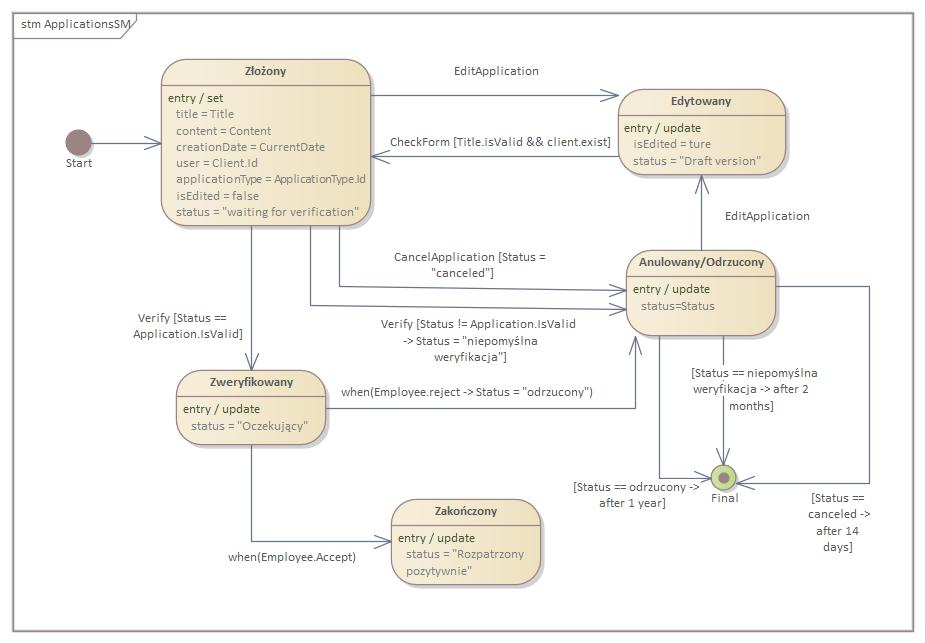
\includegraphics[width=0.7\textwidth]{images/Wniosek.jpg}
	\caption{Diagram stanów składania wniosku}
	\label{fig:StateMachine}
\end{figure}
\section{Diagramy sekwencji}
Diagram sekwencji (ang. \textit{sequence diagram}) jest uzupełnieniem diagramu klas, który reprezentuje statyczną strukturę systemu. Diagram sekwencji w dynamiczny sposób przedstawia zachowanie klas, interfejsów oraz możliwe zastosowanie metod.
\begin{figure}[H]
	\centering
	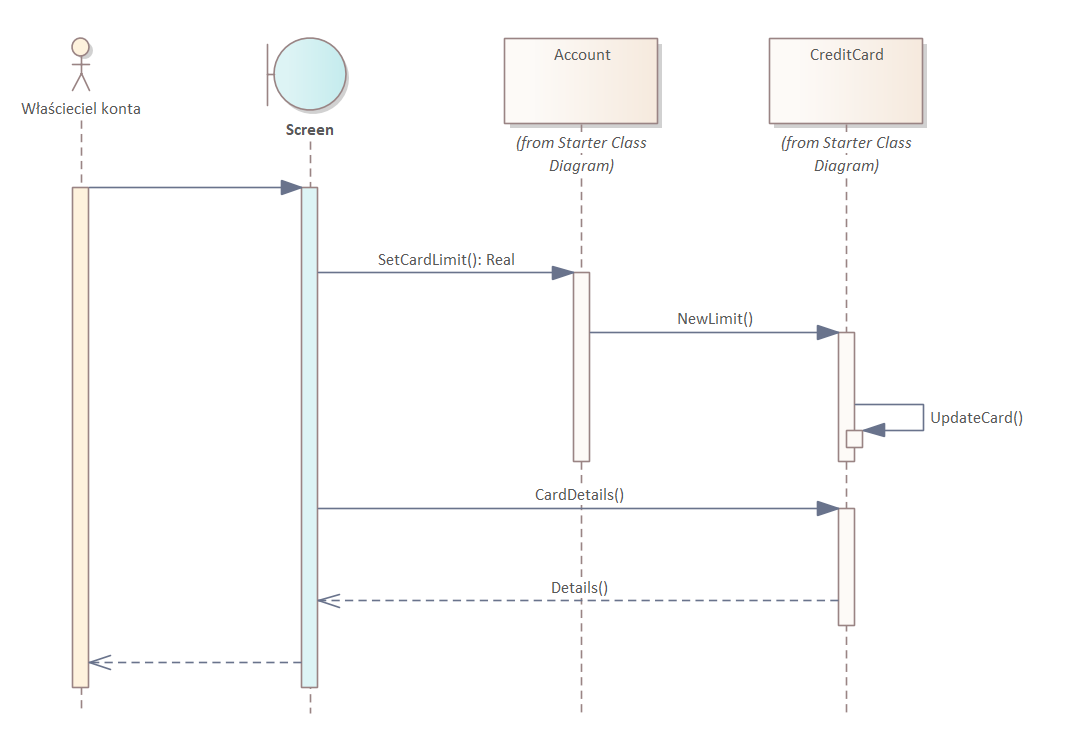
\includegraphics[width=0.7\textwidth]{images/Limit.png}
	\caption{Diagram sekwencji Limit}
	\label{fig:Seq1}
\end{figure}
\begin{figure}[H]
	\centering
	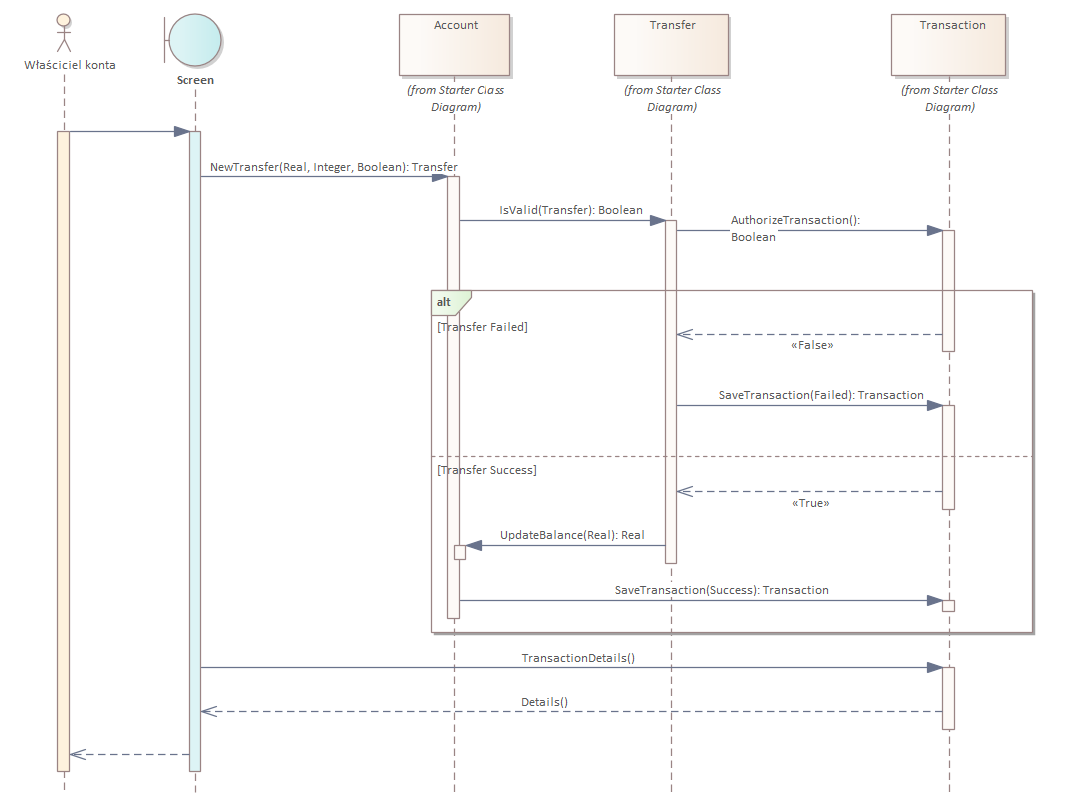
\includegraphics[width=0.7\textwidth]{images/Przelew.png}
	\caption{Diagram sekwencji Przelew}
	\label{fig:Seq2}
\end{figure}